\documentclass[preview]{standalone}
\usepackage{tkz-graph}
\begin{document}

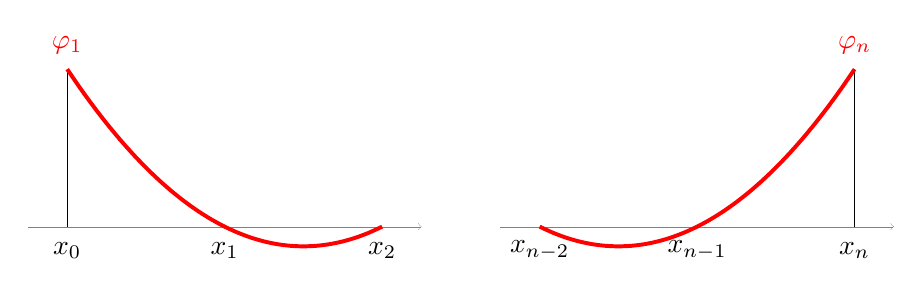
\begin{tikzpicture}
\draw[->,ultra  thin,color=gray] (1.5,0) -- (6.5, 0);
\draw[line width=0.1mm, color=black] (2,0) -- (2, 2);
\draw[red, line width = 0.5mm]   plot[smooth,domain=2:6] (\x, {- 0.5*(\x-4) + 0.25*(\x-4)^2});
\draw[red] (2, 2.3) node {$\varphi_{1}$};
\draw (2, -0.3) node {$x_{0}$};
\draw (4, -0.3) node {$x_{1}$};
\draw (6, -0.3) node {$x_{2}$};
\draw[->,ultra  thin,color=gray] (7.5,0) -- (12.5, 0);
\draw[line width=0.1mm, color=black] (12,0) -- (12, 2);
\draw[red, line width = 0.5mm]   plot[smooth,domain=8:12] (\x, {- 0.5*(\x-8) + 0.25*(\x-8)^2});
\draw[red] (12, 2.3) node {$\varphi_{n}$};
\draw (8, -0.3) node {$x_{n-2}$};
\draw (10, -0.3) node {$x_{n-1}$};
\draw (12, -0.3) node {$x_{n}$};
\end{tikzpicture}

\end{document}



После: convert pdf to png
https://convertio.co/pdf-png/



 






